

%%%%%%%%%%%%%%%%%%%%%%%%%%%%%%%%%%%%%%%%%
% University/School Laboratory Report
% LaTeX Template
% Version 3.1 (25/3/14)
%
% This template has been downloaded from:
% http://www.LaTeXTemplates.com
%
% Original author:
% Linux and Unix Users Group at Virginia Tech Wiki 
% (https://vtluug.org/wiki/Example_LaTeX_chem_lab_report)
%
% License:
% CC BY-NC-SA 3.0 (http://creativecommons.org/licenses/by-nc-sa/3.0/)
%
%%%%%%%%%%%%%%%%%%%%%%%%%%%%%%%%%%%%%%%%%

%----------------------------------------------------------------------------------------
%	PACKAGES AND DOCUMENT CONFIGURATIONS
%----------------------------------------------------------------------------------------

\documentclass{article}

\usepackage[version=3]{mhchem} % Package for chemical equation typesetting
\usepackage{siunitx} % Provides the \SI{}{} and \si{} command for typesetting SI units
\usepackage{graphicx} % Required for the inclusion of images
\usepackage{natbib} % Required to change bibliography style to APA
\usepackage{amsmath} % Required for some math elements 
\usepackage{listings}
\usepackage{color}
\usepackage{caption}
\usepackage{rotating}
\usepackage{enumitem}


\definecolor{dkgreen}{rgb}{0,0.6,0}
\definecolor{gray}{rgb}{0.5,0.5,0.5}
\definecolor{mauve}{rgb}{0.58,0,0.82}

\lstset{frame=tb,
  language=Java,
  aboveskip=3mm,
  belowskip=3mm,
  showstringspaces=false,
  columns=flexible,
  basicstyle={\small\ttfamily},
  numbers=none,
  numberstyle=\tiny\color{gray},
  keywordstyle=\color{blue},
  commentstyle=\color{dkgreen},
  stringstyle=\color{mauve},
  breaklines=true,
  breakatwhitespace=true,
  tabsize=3
}
\setlength\parindent{0pt} % Removes all indentation from paragraphs

\renewcommand{\labelenumi}{\alph{enumi}.} % Make numbering in the enumerate environment by letter rather than number (e.g. section 6)

%\usepackage{times} % Uncomment to use the Times New Roman font

%----------------------------------------------------s------------------------------------
%	DOCUMENT INFORMATION
%----------------------------------------------------------------------------------------

\title{Laboratory Assignment 5 Write Up \\ Computer Science 441} % Title

\author{\textsc{Andreas Bach Landgrebe} \\
\textsc{Andre Bryan}} % Author name

\date{\today} % Date for the report

\begin{document}

\maketitle % Insert the title, author and date

\begin{center}
\begin{tabular}{l r}
Date Submitted:  February 29, 2016 \\ % Date the experiment was performed
Partners:  Andreas Bach Landgrebe \& Andre Bryan \\ % Partner names
Instructor:  Dr. Gregory M. Kapfhammer  % Instructor/supervisor
\end{tabular}
\end{center}

% If you wish to include an abstract, uncomment the lines below
% \begin{abstract}
% Abstract text
% \end{abstract}

%----------------------------------------------------------------------------------------
%	SECTION 1
%----------------------------------------------------------------------------------------

\section{The well-commented source code of the Java classes that form the two ``useful” benchmarks.}

ShuffleClient.java

\begin{lstlisting}
import java.util.Vector;
import java.util.Random;
import org.apache.xmlrpc.*;
import java.io.*;

public class ShuffleClient {

  // The location of our server.
  private final static String server_url = "http://localhost:12345/RPC2"; 
  static String holder;
  
  public static void main (String [] args) {
    long start_val, end_val;
    Random r = new Random();
    holder = args[0];
    try {
      //Identify the server
      XmlRpcClient server = new XmlRpcClient(server_url);

      //Build Parameter Vector
      Vector params = new Vector();
      params.addElement((Object) new String(holder)); //adds command line argument to the vector

      System.out.println("Transmitting: " + params);

      start_val = System.currentTimeMillis();
      
      Object v = server.execute("fact.Shuffle", params);
      end_val = System.currentTimeMillis();
      try {
        BufferedWriter out = new BufferedWriter(new FileWriter("ShuffleClienttimes", true));
        out.write((((double)end_val-start_val)/1000)+", ");
        out.close();
      }
      catch(IOException e) {
      }
    
      System.out.println("Received: " + v);
    }

    catch (XmlRpcException exception) {
      System.err.println("JavaClient: XML-RPC Fault #" +
          Integer.toString(exception.code) + ": " +
          exception.toString());
    }
    catch (Exception exception) {
      System.err.println("JavaClient: " + exception.toString());
    }
  }
}

\end{lstlisting}

ShuffleServer.java
\begin{lstlisting}
import org.apache.xmlrpc.*;
import java.util.*;
import java.io.*;

public class ShuffleServer {

  public ShuffleServer() {
  }

  public Vector Shuffle(String x) {

    System.out.println("Received: " + x);

    //Create a vector with initial capacity of 32,000
    Vector shuffle = new Vector(0);
   for(int i =0; i <x.length(); i++){
      shuffle.addElement(new String("" + x.charAt(i)));// picks the character and adds to the vector
   }
    
    Collections.shuffle(shuffle); // shuffles the elements in the vector
    System.out.println("Returning: " + shuffle);

    return shuffle;
  }

  public static void main(String [] args) {
    long start, stop;
    start = System.currentTimeMillis();
    try {
      // Invoke me as http://localhost:12345/RPC2
      WebServer server = new WebServer(12345);
      server.addHandler("fact", new ShuffleServer());
      server.start();
    }
    catch (Exception exception) {
      System.err.println("JavaServer: " + exception.toString());
    }
    stop = System.currentTimeMillis();
    try {
      BufferedWriter out = new BufferedWriter(new FileWriter("ShuffleServertimes", true));
      out.write((((double)stop-start)/1000)+"\n");
      out.close();
    }
    catch(IOException e) {
    }
  }
}
\end{lstlisting}

%----------------------------------------------------------------------------------------
%	SECTION 2
%----------------------------------------------------------------------------------------

\section{The well-commented source code of the Java classes for the four ``baseline” benchmarks.}

FactorizationXMLClient.java

\begin{lstlisting}
import java.util.Vector;
import java.util.Random;
import org.apache.xmlrpc.*;
import java.io.*;

public class FactorizationXMLClient {

  // The location of our server.
  private final static String server_url = "http://localhost:12345/RPC2";

  public static void main (String [] args) {

    long start_val, end_val;
    //data types being used to calculate how long it takes the server to perform its task.
    Random r = new Random();
    //random generator

    try {
      //Identify the server
      XmlRpcClient server = new XmlRpcClient(server_url);

      //Build Parameter Vector
      Vector params = new Vector();
      params.addElement((Object) new Integer(r.nextInt(100)));
      //adding a random number to later find the factors of.
      //That calculation is being conducted on the server side.
      System.out.println("Transmitting: " + params);

      start_val = System.currentTimeMillis();
      //start the timing
      Vector v = ((Vector) server.execute("fact.Factors", params));
      //the server executing its task using a vector
      end_val = System.currentTimeMillis();
      //end the timing
      try {
        BufferedWriter out = new BufferedWriter(new FileWriter("ctimes", true));
        //output how long it took for the server to complete its task.
        //This is being outputting to a text document called ctimes.txt
        out.write((((double)end_val-start_val)/1000)+", ");
        //writing the output in seconds versus milliseconds
        out.close();
        //close the output stream like a good boy
      }
      catch(IOException e) {
      }

      System.out.println("Received: " + v);
      //this is the number being received from the server
    }

    catch (XmlRpcException exception) {
      //catch the exception if the connection does not go right
      System.err.println("JavaClient: XML-RPC Fault #" +
          Integer.toString(exception.code) + ": " +
          exception.toString());
    }
    catch (Exception exception) {
      System.err.println("JavaClient: " + exception.toString());
    }
  }
}
\end{lstlisting}

FactorizationXMLServer.java

\begin{lstlisting}
import org.apache.xmlrpc.*;
import java.util.*;
import java.io.*;

public class FactorizationXMLServer {

  public FactorizationXMLServer() {
  }

  public Vector Factors(int x) {

    System.out.println("Received: " + x);
    //the number being received from the client

    //Create a vector with initial capacity of 32,000
    Vector factors = new Vector(0);

    //Find the factors of x
    for (int i = 1; i <= x; i++){
      if ((x % i) == 0){
        factors.addElement((Object) new Integer(i));
      }
    }
    //returning the factors of the random number from the client
    System.out.println("Returning: " + factors);

    return factors;
  }

  public static void main(String [] args) {
    //data types being used to calculate how long it takes the server to complete its task.
    long start, stop;
    //start the timing
    start = System.currentTimeMillis();
    try {
      // Invoke me as http://localhost:12345/RPC2
      WebServer server = new WebServer(12345);
      //start the server
      server.addHandler("fact", new FactorizationXMLServer());
      server.start();
    }
    catch (Exception exception) {
      //catch any exceptions
      System.err.println("JavaServer: " + exception.toString());
    }
    //stop the timing
    stop = System.currentTimeMillis();
    try {
      //output how long it took the server to do its thing to a text document called stimes.txt
      BufferedWriter out = new BufferedWriter(new FileWriter("stimes", true));
      //write the output in seconds instead of milliseconds.
      out.write((((double)stop-start)/1000)+"\n");
      //close the output stream like a good boy.
      out.close();
    }
    catch(IOException e) {
    }
  }
}
\end{lstlisting}

LLXMLClient.java

\begin{lstlisting}
import java.util.Vector;
import java.util.Random;
import org.apache.xmlrpc.*;
import java.io.*;

public class LLXMLClient {

  // The location of our server.
  private final static String server_url = "http://localhost:12345/RPC2";
static String holder;
  public static void main (String [] args) {
    long start_val, end_val;
    Random r = new Random();
    holder = args[0];

    try {
      //Identify the server
      XmlRpcClient server = new XmlRpcClient(server_url);

      //Build Parameter Vector
      Vector params = new Vector();
      
     params.addElement((Object) new String( holder + holder + holder + holder + holder + holder));
    
      System.out.println("Transmitting: " + params);

      start_val = System.currentTimeMillis();
      Object v =  server.execute("fact.Expand", params);
      end_val = System.currentTimeMillis();
      try {
        BufferedWriter out = new BufferedWriter(new FileWriter("LLClienttimes", true));
        out.write((((double)end_val-start_val)/1000)+", ");
        out.close();
      }
      catch(IOException e) {

      }

      System.out.println("Received: " + v);
    }

    catch (XmlRpcException exception) {
      System.err.println("JavaClient: XML-RPC Fault #" +
          Integer.toString(exception.code) + ": " +
          exception.toString());
    }
    catch (Exception exception) {
      System.err.println("JavaClient: " + exception.toString());
    }
  }
}

\end{lstlisting}

LLXMLServer.java

\begin{lstlisting}
import org.apache.xmlrpc.*;
import java.util.*;
import java.io.*;

public class LLXMLServer {

  public LLXMLServer() {
  }

  public Vector Expand(String x) {

    System.out.println("Received: " + x);

    //Create a vector with initial capacity of 32,000
    Vector expand = new Vector(0);
   for(int i =0; i <10; i++){ // string concatinate 10 times
    x = x +x;
   }
     expand.addElement(new String(""+ x));

    System.out.println("Returning: " + expand);

    return expand;
  }

  public static void main(String [] args) {
    long start, stop;
    start = System.currentTimeMillis();
    try {
      // Invoke me as http://localhost:12345/RPC2
      WebServer server = new WebServer(12345);
      server.addHandler("fact", new LLXMLServer());
      server.start();
    }
    catch (Exception exception) {
      System.err.println("JavaServer: " + exception.toString());
    }
    stop = System.currentTimeMillis();
    try {
      BufferedWriter out = new BufferedWriter(new FileWriter("LLServertimes", true));
      out.write((((double)stop-start)/1000)+"\n");
      out.close();
    }
    catch(IOException e) {
    }
  }
}

\end{lstlisting}

LSXMLClient.java

\begin{lstlisting}
import java.util.Vector;
import java.util.Random;
import org.apache.xmlrpc.*;
import java.io.*;

public class LSXMLClient {

  // The location of our server.
  private final static String server_url = "http://localhost:12345/RPC2";
static String holder;
  public static void main (String [] args) {
    long start_val, end_val;
    Random r = new Random();
     holder = args[0];

    try {
      //Identify the server
      XmlRpcClient server = new XmlRpcClient(server_url);

      //Build Parameter Vector
      Vector params = new Vector();
      params.addElement((Object) new String(holder);// adds argument to the vector    
      System.out.println("Transmitting: " + params);

      start_val = System.currentTimeMillis();
      Object v =  server.execute("fact.FirstL", params);
      end_val = System.currentTimeMillis();
      try {
        BufferedWriter out = new BufferedWriter(new FileWriter("LSClienttimes", true));
        out.write((((double)end_val-start_val)/1000)+", ");
        out.close();
      }
      catch(IOException e) {
      }

      System.out.println("Received: " + v);
    }

    catch (XmlRpcException exception) {
      System.err.println("JavaClient: XML-RPC Fault #" +
          Integer.toString(exception.code) + ": " +
          exception.toString());
    }
    catch (Exception exception) {
      System.err.println("JavaClient: " + exception.toString());
    }
  }
}
\end{lstlisting}

LSXMLServer.java

\begin{lstlisting}
import org.apache.xmlrpc.*;
import java.util.*;
import java.io.*;

public class LSXMLServer {

  public LSXMLServer() {
  }

  public Vector FirstL(String x) {
    System.out.println("Received: " + x);


    //Create a vector with initial capacity of 32,000
    Vector first = new Vector(0);

    first.addElement(new String(""+ x.charAt(0)));// gets first character in the string and adds it to the vector

    System.out.println("Returning: " + first);

    return first;
  }

  public static void main(String [] args) {
    long start, stop;
    start = System.currentTimeMillis();
    try {
      // Invoke me as http://localhost:12345/RPC2
      WebServer server = new WebServer(12345);
      server.addHandler("fact", new LSXMLServer());
      server.start();
    }
    catch (Exception exception) {
      System.err.println("JavaServer: " + exception.toString());
    }
    stop = System.currentTimeMillis();
    try {
      BufferedWriter out = new BufferedWriter(new FileWriter("LSServertimes", true));
      out.write((((double)stop-start)/1000)+"\n");
      out.close();
    }
    catch(IOException e) {
    }
  }
}

\end{lstlisting}

SLXMLClient.java

\begin{lstlisting}
import java.util.Vector;
import java.util.Random;
import org.apache.xmlrpc.*;
import java.io.*;

public class SLXMLClient {

  // The location of our server.
  private final static String server_url = "http://localhost:12345/RPC2";

  public static void main (String [] args) {
    long start_val, end_val;
    Random r = new Random();

    try {
      //Identify the server
      XmlRpcClient server = new XmlRpcClient(server_url);

      //Build Parameter Vector
      Vector params = new Vector();
      params.addElement((Object) new Integer(r.nextInt(100)));// picks a random int from 0-99

      System.out.println("Transmitting: " + params);

      start_val = System.currentTimeMillis();
      Vector v = ((Vector) server.execute("fact.Before", params));
      end_val = System.currentTimeMillis();
      try {
        BufferedWriter out = new BufferedWriter(new FileWriter("SLClienttimes", true));
        out.write((((double)end_val-start_val)/1000)+", ");
        out.close();
      }
      catch(IOException e) {
      }

      System.out.println("Received: " + v);
    }

    catch (XmlRpcException exception) {
      System.err.println("JavaClient: XML-RPC Fault #" +
          Integer.toString(exception.code) + ": " +
          exception.toString());
    }
    catch (Exception exception) {
      System.err.println("JavaClient: " + exception.toString());
    }
  }
}
\end{lstlisting}

SLXMLServer.java

\begin{lstlisting}
import org.apache.xmlrpc.*;
import java.util.*;
import java.io.*;

public class SLXMLServer {

  public SLXMLServer() {
  }

  public Vector Before(int x) {

    System.out.println("Received: " + x);

    //Create a vector with initial capacity of 32,000
    Vector before = new Vector(0);
    for(int i = 0; i <x; i++){
    before.addElement((Object) new Integer(x-i));// adds every number before x to the vector
    }

    System.out.println("Returning: " + before);

    return before;
  }

  public static void main(String [] args) {
    long start, stop;
    start = System.currentTimeMillis();
    try {
      // Invoke me as http://localhost:12345/RPC2
      WebServer server = new WebServer(12345);
      server.addHandler("fact", new SLXMLServer());
      server.start();
    }
    catch (Exception exception) {
      System.err.println("JavaServer: " + exception.toString());
    }
    stop = System.currentTimeMillis();
    try {
      BufferedWriter out = new BufferedWriter(new FileWriter("SLServertimes", true));
      out.write((((double)stop-start)/1000)+"\n");
      out.close();
    }
    catch(IOException e) {
    }
  }
}
\end{lstlisting}

SSXMLClient.java

\begin{lstlisting}
import java.util.Vector;
import java.util.Random;
import org.apache.xmlrpc.*;
import java.io.*;

public class SSXMLClient {

  // The location of our server.
  private final static String server_url = "http://localhost:12345/RPC2";

  public static void main (String [] args) {
    long start_val, end_val;
    Random r = new Random();

    try {
      //Identify the server
      XmlRpcClient server = new XmlRpcClient(server_url);

      //Build Parameter Vector
      Vector params = new Vector();
      params.addElement((Object) new Integer(r.nextInt(100))); // picks random int from 0-99

      System.out.println("Transmitting: " + params);

      start_val = System.currentTimeMillis();
      Vector v = ((Vector) server.execute("fact.Product", params));
      end_val = System.currentTimeMillis();
      try {
        BufferedWriter out = new BufferedWriter(new FileWriter("SSClienttimes", true));
        out.write((((double)end_val-start_val)/1000)+", ");
        out.close();
      }
      catch(IOException e) {
      }

      System.out.println("Received: " + v);
    }

    catch (XmlRpcException exception) {
      System.err.println("JavaClient: XML-RPC Fault #" +
          Integer.toString(exception.code) + ": " +
          exception.toString());
    }
    catch (Exception exception) {
      System.err.println("JavaClient: " + exception.toString());
    }
  }
}
\end{lstlisting}

SSXMLServer.java

\begin{lstlisting}
import org.apache.xmlrpc.*;
import java.util.*;
import java.io.*;

public class SSXMLServer {

  public SSXMLServer() {
  }

  public Vector Product(int x) {

    System.out.println("Received: " + x);

    //Create a vector with initial capacity of 32,000
    Vector product = new Vector(0);

    product.addElement((Object) new Integer(x*x)); // multiplies parameter by iteself and adds it to the vector
      
    

    System.out.println("Returning: " + product);

    return product;
  }

  public static void main(String [] args) {
    long start, stop;
    start = System.currentTimeMillis();
    try {
      // Invoke me as http://localhost:12345/RPC2
      WebServer server = new WebServer(12345);
      server.addHandler("fact", new SSXMLServer());
      server.start();
    }
    catch (Exception exception) {
      System.err.println("JavaServer: " + exception.toString());
    }
    stop = System.currentTimeMillis();
    try {
      BufferedWriter out = new BufferedWriter(new FileWriter("SSServertimes", true));
      out.write((((double)stop-start)/1000)+"\n");
      out.close();
    }
    catch(IOException e) {
    }
  }
}
\end{lstlisting}

%----------------------------------------------------------------------------------------
%	SECTION 3
%----------------------------------------------------------------------------------------
\section{Using both text and diagrams, a description of client-server communication with XML-RPC.}

%----------------------------------------------------------------------------------------
%	SECTION 4
%----------------------------------------------------------------------------------------

In order to provide a detailed description of the client-server communication with XML-RPC, it is important to understand what XML and RPC and the purposes are in real world application. XML is a eXtensible Markup Language. This language is mark up language being used to define a set of rules for encoding documents. RPC is a remote procedure call. This is a computer program that causes a procedure to execute in another address space. The below diagram illustrates the client-server communication with XML-RPC \cite{tanenbaum_steen_2007}.  

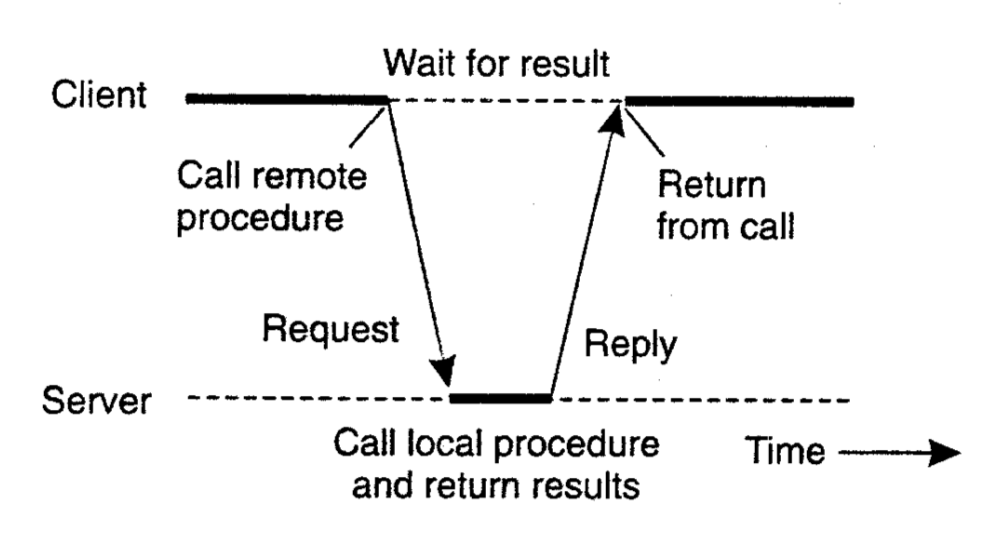
\includegraphics[scale=0.35]{XML-RPC.png}

The above diagram illustrates the principle of RPC between a client and server program. This principle does not ask the operating system to give it data. This principle packs the parameters into a message and requests that message to be sent to the server \cite{tanenbaum_steen_2007}. The first event that occurs is that client requests a call remote procedure to the server. As the client makes this request to the server, the server then makes a call to the local procedure and return results. After the server return the results, it makes a reply and return from the call to the client. 

\par

The following list best describes the steps used to summarize a remote procedure call \cite{tanenbaum_steen_2007}.

\begin{enumerate}
\item The client procedure calls the client stub in the normal way.
\item The client stub builds a message and calls the local operating system
\item The client's OS sends the message to the remote OS.
\item The remote OS gives the message to the server stub.
\item The server stub unpacks the parameters and calls the server.
\item The server does the work and returns the results to the stub.
\item The server stub packs it in a message and calls its local OS.
\item The server's OS sends the message to the client's OS.
\item The client's OS gives the message to the client stub.
\item The stub unpacks and results and returns to the client.
\end{enumerate}


\section{A detailed paper that reports on the empirical results arising from the use of the benchmarks.}

\subsection{ShuffleXML.png}

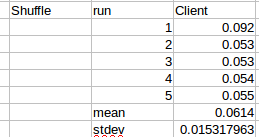
\includegraphics[scale=1.0]{ShuffleXML.png}

\subsection{LLXML.png}

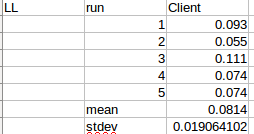
\includegraphics[scale=1.0]{LLXML.png}

\subsection{LSXML.png}

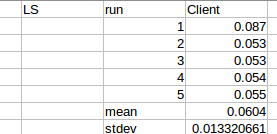
\includegraphics[scale=1.0]{LSXML.png}

\subsection{SLXML.png}

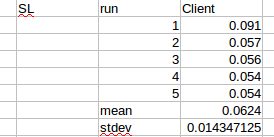
\includegraphics[scale=1.0]{SLXML.png}

\subsection{SSXML.png}

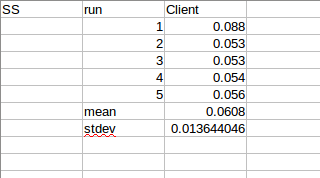
\includegraphics[scale=1.0]{SSXML.png}

\subsection{Empirical Results}
Looking at the analysis and timings from the XML Client Server lab I can see that the timings are a lot close together than the previous socket labs. Then again the same number of information was not sent over the network in the XMLRPC lab compared to the Socket lab. For the most part the timings hovered around 0.061 seconds. As you can see the average run times for all of the different client and server sizes did not change tremendously from the increase in the size of hat was sent over the network. For instance, the Small Client and Small Server  had an average run time of 0.0608 and the Small Client and Large Server had a mean of 0.0624. That is a very small increase in run time. Then we look at a Large Client and Small Server then mean was at 0.0604 which is actually faster than the time of a Small Client and Small Server. A Large Client and Large Server was .0814. Even then it is still not a big increase in the timing of the different sizes of the XMLRPC Servers and Clients. Then there is the Shuffle Client and Server that was created that shuffles the input from the command line. The average timing for the client and server turned out to be 0.0614. Comparing this lab to the Socket lab I can say that it wasn't as fun using XMLRPC in comparison to using Sockets in java. It was just a lot more annoying and I ran in to a lot of errors with casting and using Vectors in Java. However, knowing how XMLRPC differs from the Socket Communication I can strongly say that if we ran the same sizes on XMLRPC the timing would differ a lot between sockets and XMLRPc and XMLRPC will run slower than Sockets because of unwrapping on both sides of the Client and Server.

%----------------------------------------------------------------------------------------
%	SECTION 5
%----------------------------------------------------------------------------------------
\section{A description of the challenges that you encountered when completing this assignment.}

There were various challenges that we had encountered when completing this assignment. One of these included receiving casting problems when implementing the useful benchmarks. In order to overcome this, we had to collaborate together and perform pair programming in order to overcome this issue. Another issue that arose during this assignment is being able to meet up. Due to one of the members being part of the tennis team and the other member being part of the track and field team, it is diffcult at times to be able to meet up to complete the work assignned for this laboratory assignment. In order to overcome, we were able to write down our contact information and collaborate together to complete this laboratory assignment. 

%----------------------------------------------------------------------------------------
%	SECTION 6
%----------------------------------------------------------------------------------------
\section{A detailed listing of the tasks completed by each member of your partnership.}
In order to complete this assignment at the correct time, dividing up the work was essential. The way we did this was by haivng Andre be repsonsible for writing the source code for the benchmarks and provide a detailed results analysis. Andreas was responsible for writing comments on the provided Java files, and giving a detailed paper explaining the client-server communication with XML-RPC.


%----------------------------------------------------------------------------------------
%	BIBLIOGRAPHY
%----------------------------------------------------------------------------------------

\nocite{tanenbaum_steen_2007}

\bibliographystyle{plain}

\bibliography{sample}

%----------------------------------------------------------------------------------------


\end{document}
